\documentclass[12pt,letterpaper, onecolumn]{exam}
\usepackage{amsmath}
\usepackage{amssymb}
\usepackage[lmargin=71pt, tmargin=1.2in]{geometry}  %For centering solution box
\lhead{Samuel Molero\\}
\rhead{Section: 501\\}
\usepackage{subcaption}
\usepackage{graphicx}
% \chead{\hline} % Un-comment to draw line below header
\thispagestyle{empty}   %For removing header/footer from page 1

\begin{document}
\begingroup  
    \centering
    \LARGE STATS 211\\
    \LARGE Homework 1 \\[0.5em]
    \large \today\\[0.5em]
    \large Samuel Molero\par
    \large samueljosemolero@tamu.edu\par
    \large Section: 501\par
\endgroup
\rule{\textwidth}{0.4pt}
\pointsdroppedatright   %Self-explanatory
\printanswers
\renewcommand{\solutiontitle}{\noindent\textbf{Ans:}\enspace}   %Replace "Ans:" with starting keyword in solution box

\begin{questions}

    \question[1 Mark] Q1 \\
    \begin{parts}
        \part Construct the (t, y) and (t, log(y)) scatter scatter ploth scatterplot suggests a linear relationship?\\
            \begin{solution}
            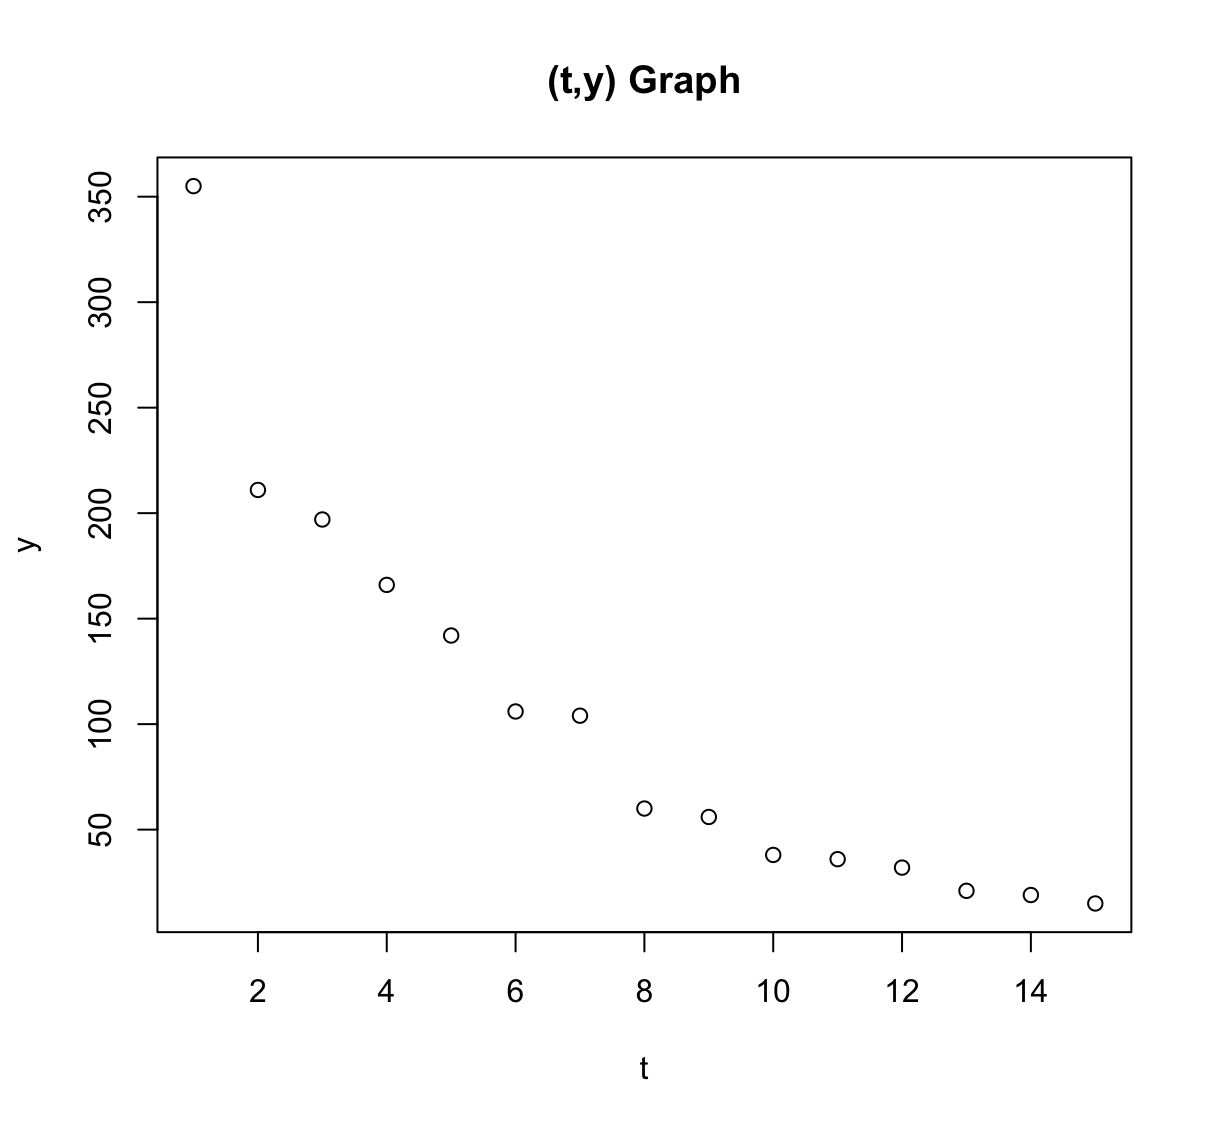
\includegraphics[width=0.4\textwidth]{Homeworks/yGraph.png} 
            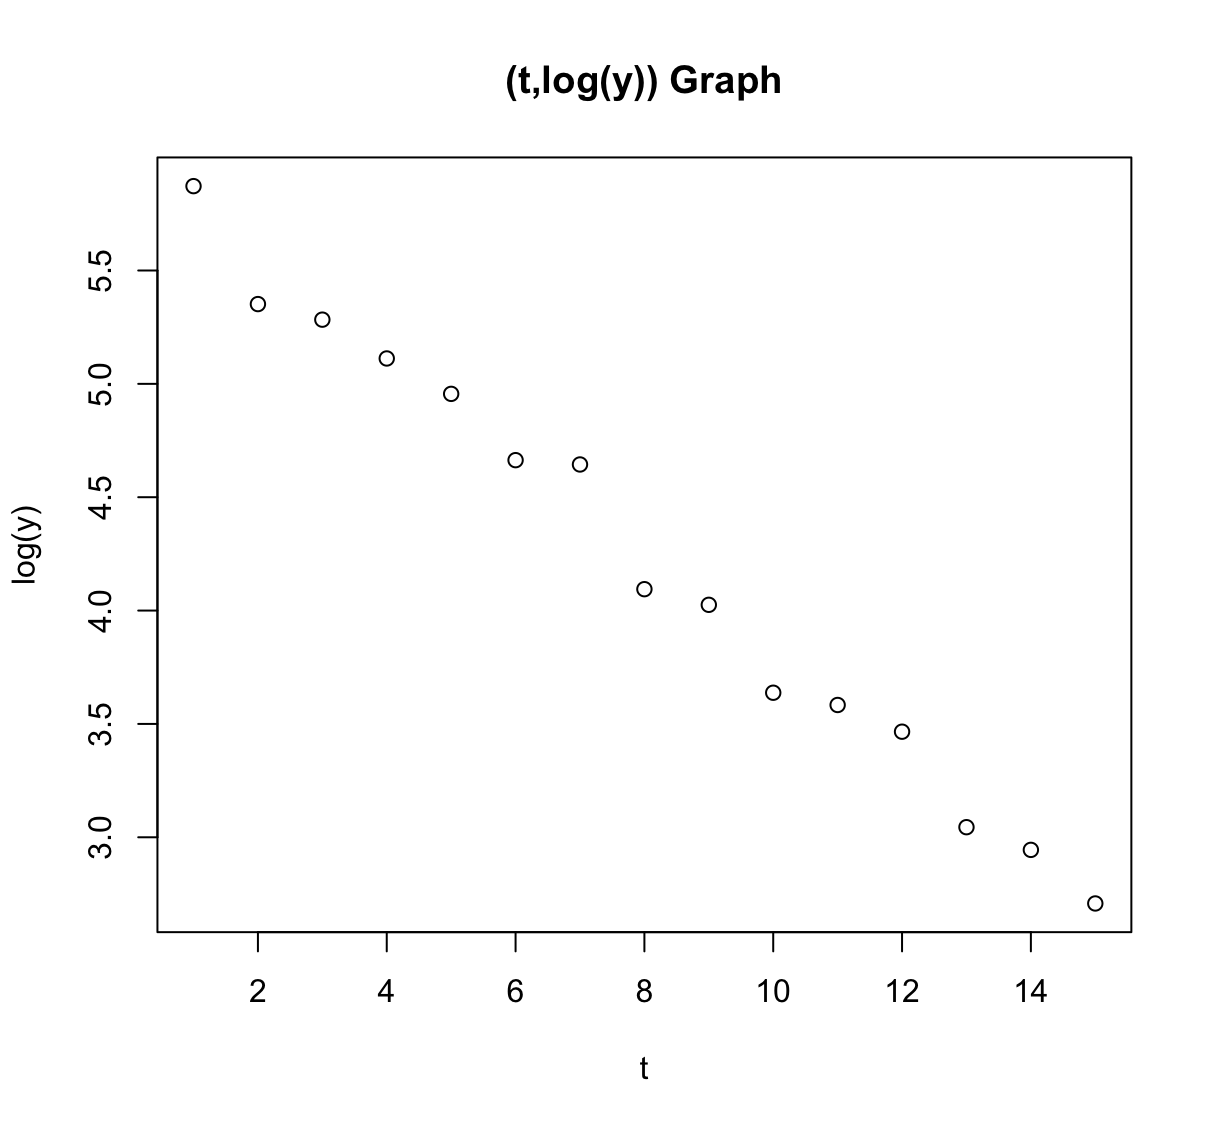
\includegraphics[width=0.4\textwidth]{Homeworks/Log(y)Graph.png} 
            \end{solution}
        \part Construct a predictive equation for the bacteria count Y at time t.
        \begin{solution}
            \begin{verbatim}
                # R code snippet
                # lm_fit <- lm(y_log~t)
                # summary(lm_fit)
            \end{verbatim}
            Using the command above will provide both the intercept and slope for the linear regression equation using the log form values of Y. Which results in the following equation:\\
            \center
            $ log(\hat{y})  = 5.9732 -0.2184t$\\
            Solving for the predictive model for bacteria count Y at time t results in:\\
            $y = e^{5.9732 -0.2184t}$
        \end{solution}
        
    \end{parts}
    
    
    \question Q2?
    
    \begin{solution}
            
        \begin{parts}
            \part 
            \part Solution for (b)
        \end{parts}
    \end{solution}

    \pagebreak %Not necessary
    
    \question[Type anything here] Q3?\droppoints
    
    \begin{solution}
            A3.
    \end{solution}
    
\end{questions}
\end{document}